\subsection{Betting System - a measure for quality control}
Many of the existing gamified systems point out the importance of quality control in \ac{gwap}. Von Ahn et al. \cite{44} suggests two mechanisms for ensuring correctness of data: player testing \footnote{Player testing is evaluating the players output by occasionally matching it against gold standards or already annotated data} and repetition or redundancy of data. In our game design we have employed two mechanisms for ensuring that the quality of annotations performed through the game is maintained. 
The first assessment methodology is accumulating multiple individual answers for a specific entity before deciding whether that answer is correct or not. This corresponds to the redundancy of data for quality control suggested by \cite{44}. The second assessment methodology is using the betting system incorporated into the game. If we look at the betting element in the game from the eyes of a game designer, this element represents the lens of triangularity proposed by Schell \cite{51} (page 212). The lens of triangularity gives a player the choice to play safe for small rewards or take a risk and win big rewards. Triangularity gives an interesting and exciting flavour to our game. On the other hand, if we look at this game element from the eyes of a linguistic expert who demands from the game the generation of trustful and qualitative annotations, than this element represents a measure for assessing the confidence of a player towards the his choice of candidate. Figure \ref{fig:game-bet} illustrates the betting screen shown to the player immediately after having completed the quiz.

\begin{figure}[]
    \centering
    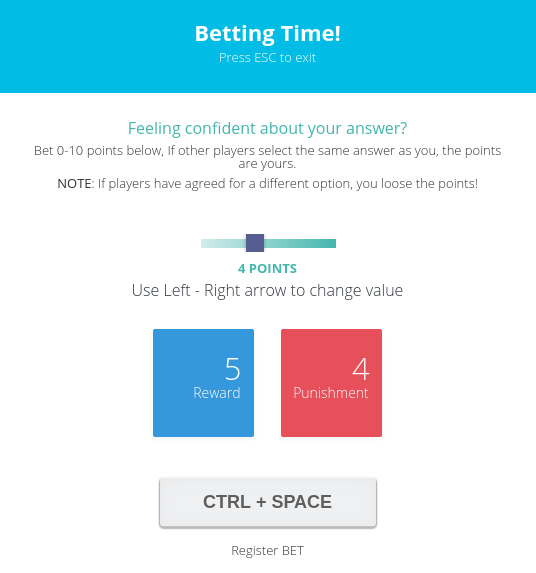
\includegraphics[width=.8\linewidth]{figures/experiment2/game-bet2.png}
    \caption{Betting Mechanism as a quality control and representative of triangularity for Fastype}
    \label{fig:game-bet}
\end{figure}

As we can see from Figure \ref{fig:game-bet}, the player has the choice of deciding the amount of points he wants to bet on the selected answer. The bigger the number of points used in the bet the higher the risk of loosing or wining them. Players are instructed to think if other players who might potentially encounter the same quiz will also choose the exact same answer as they did. In that case, if they are confident about the given answer, then the players are encouraged to place high bets rather than playing it safe. However, the choice remains completely in the hands of the player. Our betting mechanism works in the way that for one individual entity, when more than 4 unique judgments agree on the same candidate, than this entity is considered to be resolved. All the players whos' selected candidate is the same as the correct candidate (meaning their answer falls within the absolute majority) will be rewarded with the amount of points they bet for the particular entity. Similarly, all the players whos' answer was not the one selected by the majority are punished by subtracting the amount of points they bet from their overall accumulated points in the game. In terms of annotation quality, candidates with higher betting scores represent higher levels of confidence which means we can be sure that the selected candidate is undoubtedly the correct representative for the target entity.